\documentclass[12pt]{article}
\usepackage{times}
\usepackage[titletoc]{appendix}
\usepackage{graphicx}
\usepackage{lineno}
\usepackage{multirow}
\usepackage[english]{babel}
\usepackage{hyperref}
\hypersetup{
    colorlinks=true,       % false: boxed links; true: colored links
    linkcolor=blue,          % color of internal links (change box color with linkbordercolor)
    citecolor=darkgreen,        % color of links to bibliography
    filecolor=magenta,      % color of file links
    urlcolor= black           % color of external links
}
\usepackage{typearea} 
\usepackage{amssymb}
\usepackage{amsfonts}
\usepackage{amsmath}
\usepackage{enumerate}
\usepackage[round,authoryear]{natbib}

\usepackage{wrapfig}
\usepackage{lscape}
\usepackage{rotating}

\renewcommand{\baselinestretch}{1.2}
\newcommand{\bbar}[1]{\overline{#1}}

\usepackage{color}
	 \definecolor{darkred}{rgb}{0.75,0,0}
	 \definecolor{darkgreen}{rgb}{0,0.5,0}
	 \definecolor{darkblue}{rgb}{0,0,0.75}
	 \definecolor{magenta}{rgb}{0,0,0.75}
\newcommand{\cha}[1]{\textcolor{darkblue}{(#1)}}
\newcommand{\marcus}[1]{\textcolor{darkred}{(#1)}}
\newcommand{\paul}[1]{\textcolor{red}{(#1)}}

\title{\vspace*{-22mm}\bf Eco-evolutionary dynamics of mutualisms}
\author{Chaitanya S. Gokhale$^{1*}$,
Marcus Frean$^{2}$,
 \and Paul B. Rainey$^{1,3}$ \\
\normalsize $^{1}$New Zealand Institute for Advanced Study, Massey University, Auckland, New Zealand, \\
\normalsize $^2$Victoria University of Wellington, Wellington, New Zealand\\
\normalsize $^3$Max Planck Institute for Evolutionary Biology, \\
\normalsize August-Thienemann-Stra{\ss}e 2, 24306 Pl\"{o}n, Germany,\\
}

\date{}

\begin{document}

%\linenumbers
\maketitle

\begin{abstract}
%Mutualisms present a conundrum for evolutionary theory.
%In the short term, a species that exploits another is likely to have a fitness advantage relative to a competitor species that shows restraint.  
%\paul{ I'm not too clear about the above sentence and whether I have captured what you intend.}
%Therefore how mutualisms emerge and are maintained over longer evolutionary time scales remains an important issue.
%Game theoretic approaches involving reciprocal interactions among species are often used to study mutualisms, however such approaches typcially neglect the importance of within species interactions.
%Separating inter and intraspecies interactions may not be always possible especially if the same individuals act within and between species.
%\paul{the above sentence does not flow nicely from the previous.}
%Feedbacks between inter and intraspecies interactions are then inevitable and need to be taken into account.
%Including population dynamics adds an ecological component to the study.
%Herein we study the full eco-evolutionary dynamics of mutualism between two species when a variety of  intraspecies interactions are possible.
%Our results show that while mutualism can turn into parasitism by overexploitation, for some intraspecies dynamics, mutualism can be maintained even while maintaining exploiters in the species composition.
%\paul{ over all the abstract is not great and it gets worse as it proceeds.  It needs to be reworked. It wants to better follow the text.  Start with between species interactions,  then add a layer of realism by incorporating within species interactions.  Another layer with time, and then density.  Then a statement of the most significant highlevel finding.  The current "Our results show..." sentence is not a killer.  It needs to be a killer sentence that does the work justice. }
\end{abstract}

\noindent
Keywords: mutualism,evolutionary game theory,multiple players, population dynamics, seasonality

\tableofcontents

\section{Introduction}
Mutualisms have long been recognised as worthy of attention and have been of critical interest over the centuries \citep{aristotle:book:350,janzen:bookchapter:1985,bronstein:book:2003}.
The study of mutualistic relationships -- interspecific interactions that benefit both species -- is a rich field of experimental, empirical and theoretical study 
\citep{boucher:book:1985,hinton:PTENHS:1951,wilson:AmNat:1983,bronstein:QRB:1994,poulin:JTB:1995,noe:book:2001,johnstone:ECL:2002,pierce:ARE:2002,kiers:Nature:2003,bergstrom:PNAS:2003,hoeksema:AmNat:2003,bshary:ASB:2004,akcay:PRSB:2007,bshary:Nature:2008,gokhale:PRSB:2012,archetti:JTB:2013}.
A typical question is what keeps mutualisms from evolving into parasitism.
The maintenance of such cooperative relationship is often attributed to compensatory mechanisms like sanctioning or rewarding.
Theoretically too it has been shown that mutualisms are hard to evolve unless bits of ecological reality are included \cite{doebeli:PNAS:1998}.
While studying mutualism most of the studies focus on understanding the interspecies interaction pattern which is clearly the object of interest.
However in nature these interactions do not occur in isolation from other levels of community interactions.
Thus including ecologically relevant factors such as intraspecies interactions, seasonality and density effects can ease the maintenance of mutualism even in presence of exploiters within each species. 


It has become increasing clear that separating evolution from ecology and studying it in isolation may provide us with a warped view of the actual eco-evolutionary trajectory \citep{sanchez:PLoSB:2013}.
The effect of seasonality and/or densities of the mutualists can be a determining factor in the maintenance of mutualisms \citep{visick:JB:2000,warren:GCB:2014,mcfallngai:PLoSB:2014}.
Evolutionary game theory provides a simple and tractable framework for anlaysing mutualism by a cost-benefit analysis of the interactions \citep{trivers:QRB:1971,weibull:book:1995,hofbauer:JMB:1996,hofbauer:book:1998}
For mutualisms, it is usually more or less clear what the benefits are.
However how can we exactly quantify the costs involved for the two species.
This difference in the cost-benefit functions for the two species needs to be taken into account when analysing the interactions.
Furthermore these costs and benefits can depend on the number of interacting individuals from the mutualistic species \citep{pierce:BES:1987,noe:TREE:1995,hoelldobler:book:1990,hill:OEC:1989,noe:book:2001,kiers:Nature:2003,stanton:AmNat:2003,stadler:book:2008,kiers:Science:2011}. 
Theoretical models have recently been developed towards this end \citep{archetti:EL:2011,archetti:JTB:2013}. 
While these developments are in the desired direction, they still lack explicit ecological effects.
It is natural to imagine that the observed mutualism may be seasonal and the interactions are not a continuous feature of the evolutionary trajectory of a species. 
Furthermore the two species can often occupy different niches and hence have different carrying capacities.
Important ecological effects such as the Allee effect would often be ignored if the population density of a species is not taken into account.


Overall we look at the broader picture of how the eco-evolutionary dynamics of mutualisms are shaped when both the inter as well as intraspecies dynamics are taken together. 
We find that including the full range of interactions provides us with a set of rich and intricate dynamics which are not possible when either one of these dimensions is ignored.
Beginning with the previously studied interspecies dynamics \citep{gokhale:PRSB:2012} we increase the complexity of the system by including seasonality.
We tackle this by varying the duration of the impact of intraspecies and interspecies dynamics.
For the complete eco-evolutionary picture to emerge we further include population dynamics.
Including such dynamics informs us about the population densities we might expect to find the interactors to evolve to.
We demonstrate the crucial nature of the feedback between population and evolutionary dynamics which can maintain mutualisms preventing either or both species from going extinct.
Mutualism, with a healthy mix of exploiters and cooperators, emerges only when the intraspecies interactions are included and persist when ecologically relaistic phenomena like seasonality and 
The rich dynamics observed provides us with novel insights about the immense asymmetries in mutualisms and the fragility of such delicately balanced interactions.


\section{Model and Results}


\begin{figure}
\begin{center}
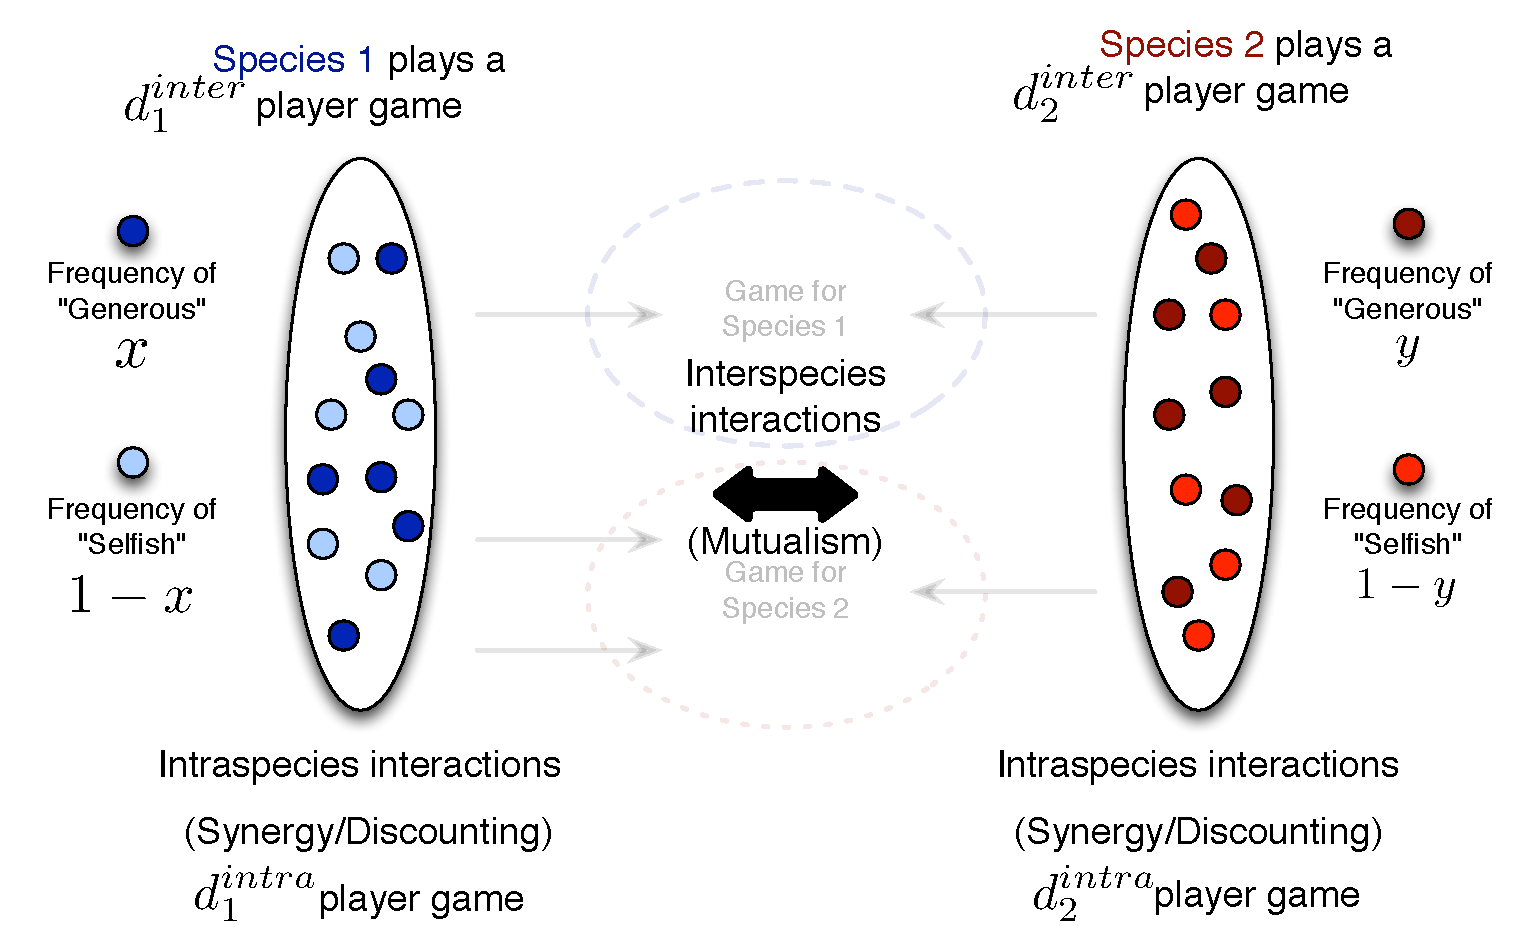
\includegraphics[scale=0.5]{Figures/interintra.pdf}
\caption{\small{
\textbf{Evolutionary dynamics with combined inter-intra-species dynamics.}
We assume the interactions between species to be mutualistic described by the snowdrift game \citep{bergstrom:PNAS:2003,souza:JTB:2009,gokhale:PRSB:2012}.
Species $1$ plays a $d_1^{inter}$ player game with species $2$ while species $2$ plays a $d_2^{inter}$ player game.
Each species has two types of players ``Generous" and ``Selfish" who besides interacting with the members of other species, also take part in intraspecies dynamics.
For intraspecies interactions we assume a general framework of synergy and discounting which can recover the \textit{classical} outcomes of evolutionary dynamics \citep{eshel:AmNat:1988,hauert:JTB:2006a,nowak:book:2006}
}
\label{fig:conceptart}
}
\end{center}
\end{figure}


\subsection{Interaction dynamics}
\subsubsection{Interspecies}

Focusing on mutualism, the interspecies dynamics is given by the multiplayer version of the snowdrift game \citep{bergstrom:PNAS:2003,souza:JTB:2009,gokhale:PRSB:2012} (also known as hawk-dove, or chicken).
A common benefit is generated by contributions from both species but there is a cost involved to it and species do not need to contribute equally. 
However the individuals in each species could get away with contributing a bit less than other individuals.
We assume that each species consists of two types of individuals ``Generous" $G$ and ``Selfish" $S$. 
If enough individuals are ``Generous" and contributing to the generation of mutual benefits then other individuals can get away with being selfish (not contributing). 
But all individuals in the game lose out if not enough are generous. Hence both species cannot be completely ``selfish", as per the definition of mutualism.
This interaction framework corresponds to that of a multiplayer version of a snowdrift game and is discussed in detail in the Supplementary Material (SI).
Hence the pressure is on a species to make the partner ``Generous" while itself being ``Selfish".
The fitness of each of the types within a species depends on the composition of the other species.
Denoting the frequency of the``Generous" types in species $1$ ($G_1$) as $x$, and that in species $2$ ($G_2$) as $y$, the fitness of $G_1$  is given by $f^{inter}_{G_1} (y)$ and that of $G_2$ as $f^{inter}_{G_2} (x)$. 

\subsubsection{Intraspecies}

For intraspecies dynamics we do not restrict ourselves to any particular interaction structure and thus make use of the general multiplayer evolutionary games framework \citep{gokhale:PNAS:2010,gokhale:DGAA:2014}.
Moving from the interspecies dynamics, the two types already described are ``Generous" and ``Selfish".
Thus we already have each species containing two different types of individuals.
It is possible that a different categorisation exists within a species.
Thus if the interactions within a species are say between ``Cooperators" and ``Defectors", these types could be made up of a combination of ``Generous" and ``Selfish" individuals.
However for the sake of simplicity we study the dynamics between ``Generous" and ``Selfish" types within a species where the types are defined at the interspecies level.
The cost benefit framework described in \citep{eshel:AmNat:1988,hauert:JTB:2006a}
 allows us to transition between four classic scenarios of evolutionary dynamics \citep{nowak:Science:2004}.
For example in our case we can have a dominance of the ``Generous" type or the ``Selfish" type or both the types can invade from rare resulting in a co-existence or bistability if both pure strategies are mutually non-invasive.
For the intraspecies interactions the fitness of a $G_1$ is then given by $f^{intra}_{G_1} (x)$ and that of $G_2$ is given by $f^{intra}_{G_2} (y)$ and similarly for the ``Selfish" types.

\subsection{Combined dynamics}

Putting together intra and interspecific dynamics provides a complete picture of the possible interactions occurring. While we are interested in mutualism at the level of the interspecies interactions there are four possible interactions within each species \citep{nowak:Science:2004,hauert:JTB:2006a} (dominance of either type, coexistence or bistability). Since the within species interactions for the two different species do not need to be the same, there are in all sixteen different possible combinations.
Assuming additivity in the fitnesses of inter and intraspecies fitnesses, the combined fitness of each of the two types in the two species are given by,

%
\begin{align}
	f_{G_1} (x,y) &= p f^{inter}_{G_1} (y) + (1-p) f^{intra}_{G_1} (x) \\
	f_{S_1} (x,y) &= p f^{inter}_{S_1} (y) + (1-p) f^{intra}_{S_1} (x)  \\
	f_{G_2} (x,y) &= p f^{inter}_{G_2} (x) + (1-p) f^{intra}_{G_2} (y) \\
	f_{S_2} (x,y) &= p f^{inter}_{S_2} (x) + (1-p) f^{intra}_{S_2} (y).
\label{eq:combinedfiteqs}
\end{align}
%
The parameter $p$ tunes the impact of each of the interactions on the final fitness that eventually drives the evolutionary dynamics.
For $p=1$ we recover the well studied case of the Red King dynamics \citep{gokhale:PRSB:2012}, while for $p=0$ the dynamics of the two species are  decoupled and can be individually studied by the synergy/discounting framework of nonlinear social dilemmas \citep{hauert:JTB:2006a}.
Of interest here is the continuum described by the intermediate values of $p$.
However that means we need to track the qualitative dynamics of sixteen possible intraspecies dynamics as $p$ changes gradually from $0$ to $1$ (Appendix \ref{app:combineddyn}). 
The time evolution of the ``Generous" types in both species is then given by,
%
\begin{align}
\dot{x} &= r_x x \left(f_{G_1}(x,y) -  \bar{f}_1(x,y) \right)  \\
\dot{y} &= r_y y \left(f_{G_2}(x,y) -  \bar{f}_2(x,y) \right).
\label{eq:repeq}
\end{align}
%
A crucial part of co-evolution is the rates of evolution \citep{salathe:TREE:2008}.
If the two species evolve at different rates (here $r_x$ for species $1$ and $r_y$ for species $2$), which is often the case, then this certainly has the potential to skew the balance of benefits away from equality in mutualism \citep{bergstrom:PNAS:2003}.
Furthermore the balance can also be affected by the number of interacting partners between the two species \citep{gokhale:PRSB:2012}.
This approach provides us with a powerful method to incorporate a multitude of realistic concepts in the analysis.
For example the number of players involved in a game, which has been shown to be a crucial factor in determining the evolutionary dynamics could be different for each interactions, inter and intraspecies interactions for species $1$ ($d^{inter}_1$, $d^{intra}_1$) and similarly for species 2 ($d^{inter}_2$, $d^{intra}_2$). 
The interspecies interactions are proxied by the multiplayer snowdrift game which can incorporate threshold effects.
For example a certain number of ``Generous" cleaner fish may be required to clean the host or a certain number of ``Generous" ants required to protect larva from predators.
We can have $M_1$ and $M_2$ as the thresholds in the two species.
Since the interaction matrices for the inter and intraspecies dynamics are completely different, in principle, we can have different costs and benefits for the four games (two snowdrift games from the perspective of each species and the intragames within each species).

We can have a diverse and rich set of dynamics possible which brings into question the study of coevolution based on only interspecies interactions. 
For a given set of parameter values but the the full spectrum of possible dynamics, see Figure \ref{fig:appendix}.
Even under a large number of assumptions and even if the intraspecies dynamics accounts for only $33\%$ ($1-p$) of the cumulative fitness, we can see drastically different qualitative dynamics which is capable of explaining the persistence of exploiters (Fig. \ref{fig:mainexampleone}).
The traditional mutualistic modeling approach can end up in the diagonal fixed points where one of the species can get away with being completely ``Selfish" while forcing the other to be ``Generous".


\begin{figure}
\begin{center}
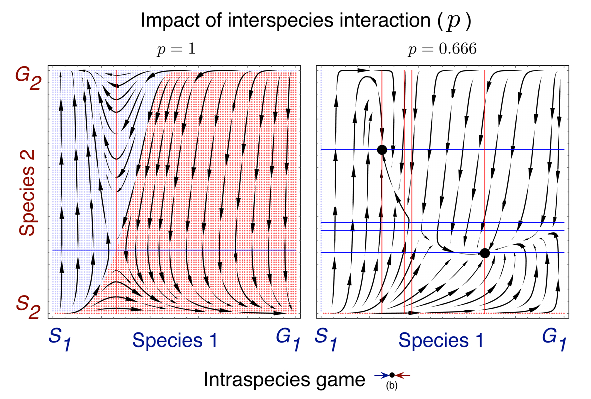
\includegraphics[width=\columnwidth]{Figures/mainexample2.pdf}
\caption{\small{
\textbf{Change in evolutionary dynamics due to inclusion of intraspecies dynamics.} When the fitness of the ``Generous" and ``Selfish" types in both the species is solely determined by the interactions which occur between species (in this case mutualism, $p=1$) then we recover the dynamics as studied previously in \citep{gokhale:PRSB:2012}. The colours represent the initial states which result in an outcome favourable for species $1$ (blue leading to ($S_1$,$G_2$)) and species $2$ (red, leading to ($G_1$,$S_2$)). This can result in the Red King effect and other possible complexities as discussed recently in \citep{gao:SciRep:2015}. However when we start including intraspecies dynamics the picture can be very different.
Even when the impact of intraspecies dynamics is only a $1/3$ on the total fitness of the ``Generous" and ``Selfish" types we see a very qualitatively different picture.
Two fixed points are observed where both the ``Generous" and ``Selfish" types can co-exist in both the species.
All initial states in the interior lead to either one of these fixed points (hence the lack of colours).
However it is still possible to characterise the ``successful" species as one of the equilibrium is favoured by one species than the other.
The horizontal isoclines are for species $1$ while the vertical ones are for species $2$.
The analysis was done for a 5 player game $d_1^{inter} = d_2^{inter} = d_1^{intra} = d_2^{intra} = 5$, $b=2$, $c=1$ and $r_x = r_y /8$ for the interspecies mutualism game while additionally $\tilde{b}_1 = \tilde{b}_2 = 10$ and $\tilde{c}_1 = \tilde{c}_2 = 1$ and $\omega_1 = \omega_2 = 3/4$ for the two intraspecies games within each species. Note that even with symmetric games within each species we can a qualitatively drastic difference when compared to the dynamics excluding intraspecies interactions.  For different intraspecies interactions within each species and for varying $p$ see SI.}
\label{fig:mainexampleone}
}
\end{center}
\end{figure}

\subsection{Seasonality}

Many mutualisms are observed only during certain periods of a year.
Such seasonal or episodic mutualism run a high risk of phenological partner mismatch as a result of climate change \citep{rafferty:Oikos:2015}.
While tropical species, such as the various varieties of fig (\textit{Ficus}) can flower all year round, their mutualistic relationships (with wasps) run a lower risk.
For example in the ant-aphid mutualism, the number of attending ants was seen to increase till June and declined after late July and the aphid colonies went rapidly (within a month) extinct in the absence of attending ants \citep{yao:Oikos:2000,yao:JIS:2009}.
For the evolution of a species this means that the effect of interspecific interaction changes over time.

To analyse such episodic mutualistic events, instead of a static variable $p$ measuring the impact of interspecific interaction on fitness we make use of a time-dependent function $p(t) = (1 + \sin(a t))/2 $.
For the particular parameter set used in Fig. \ref{fig:mainexampleone} ($p=0.666$ panel), introducing seasonality still maintains the two interior fixed points (they are closer to each other for $p = 0.5$), but this is seen only when the oscillations in $p(t)$  are comparable, $a=1$, or faster, $a=10$, with respect to the evolutionary timescale.
For slower oscillations $a=0.1$ we see cyclic behaviour which is prominent in species $2$ more than in species $1$.
Slow oscillations mean that the system spends longer close to the starting value of $p(t)$ and hence the phase in which $p(t)$ starts becomes more and more important for smaller and smaller $a$. 
This is especially interesting if the stability of the system is qualitatively affected over the $p$ continuum.


\begin{figure}
\begin{center}
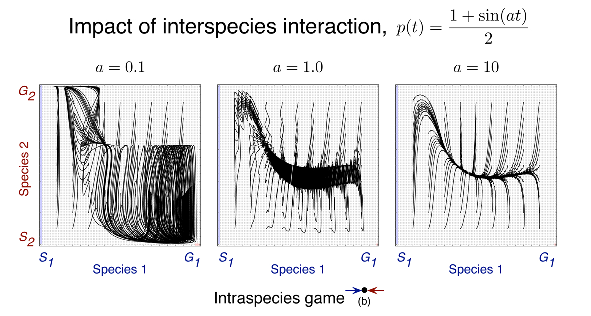
\includegraphics[width=\columnwidth]{Figures/oscillating_p_reduced.pdf}
\caption{\small{
\textbf{Seasonal changes in the interspecies interactions affecting the evolutionary dynamics within species.}
We model the impact of the interspecies interaction on the fitness of the different types as in Eqs.~\ref{eq:combinedfiteqs} however instead of a static value for $p$ we introduce seasonality via a simple sine function as $p(t) = (1+\sin(at))/2$.
Here, $a$ denotes how the seasonality time scale relates to the inter-intra-species interactions timescale.
A large $a$ denotes multiple bouts of mutualism affecting fitness for a given evolutionary time step while a small $a$ denotes fewer of such bouts within the same evolutionary time step.
The trajectories shown in the panels are obtained by numerical interactions with initial conditions $x = y = \{0.1,0.9\}$ and a step size of $\Delta x = \Delta y = 0.1$.
The background colour is obtained by a finer grain of $\Delta x = \Delta y = 0.01$ and depict the same outcomes as in Fig. \ref{fig:mainexampleone}, with gray representing the outcome that none of the edge equilibria are reached.
For comparable or larger $a$ the dynamics under oscillations can be captured by the average dynamics (at $p = 0.5$) however for small $a$ we a see qualitatively different outcome.
Furthermore the phase in which the oscillating function begins is more important for smaller and smaller $a$ especially if the stability of the fixed points changes as $p$ changes (see Fig. \ref{fig:appendix} panel (b) x (b) across the $p$ continuum).
 }
\label{fig:oscillations}
}
\end{center}
\end{figure}


\subsection{Population dynamics}

Until now we have considered that each species consists of two types of individuals and they make up the population of that species.
However populations sizes change over time. 
Assuming that ecological changes are fast enough that they can be averaged out, we can usually ignore their effect on the evolutionary dynamics.
It is now possible to show that evolution can happen at fast timescales, comparable to those of the ecological dynamics \citep{post:PTRSB:2009,beaumont:Nature:2009,hanski:PNAS:2011,sanchez:PLoSB:2013}.
Hence we need to tackle not just evolutionary but eco-evolutionary dynamics together.
%
\begin{figure}
\begin{center}
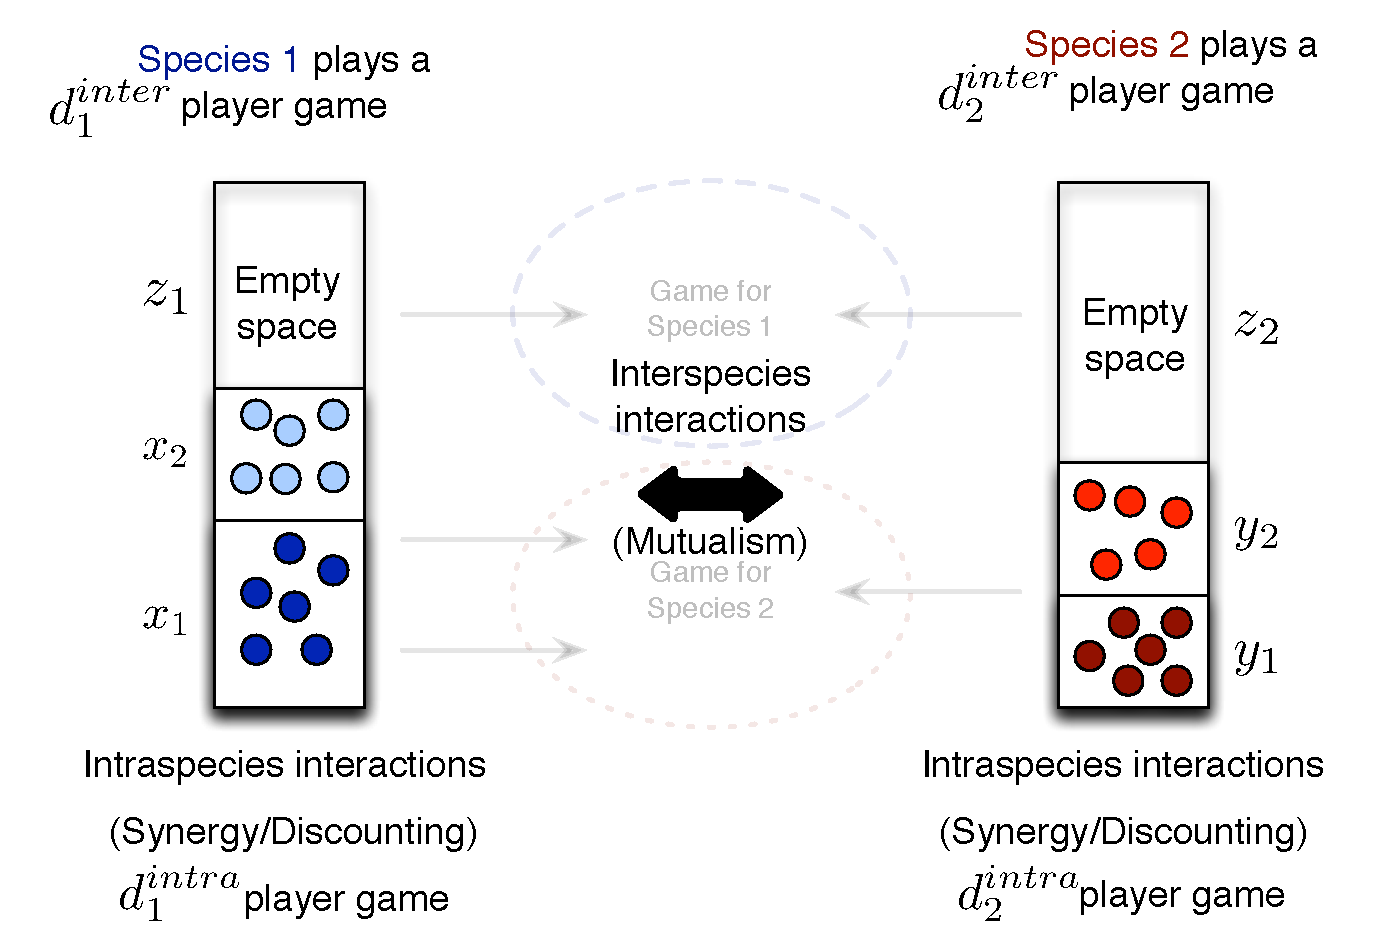
\includegraphics[scale=0.5]{Figures/popdyninterintra.pdf}
\caption{\small{
\textbf{Population and evolutionary dynamics with combined inter-intra-species dynamics.}
As with the interactions described in Fig. \ref{fig:conceptart} the two species consist of two types of individuals ``Generous" and ``Selfish".
Since the two species can in principle occupy different environmental niches, they  can have non-overlapping population carrying capacities.
The normalised carrying capacity in both species is $1$ and we have $x_1 + x_2 + z_1 = 1$ (for species $1$) where $x_1$ and $x_2$ are the densities of the ``Generous" and ``Selfish" types respectively (similarly with $y$ and $z_2$ in species $2$). 
The parameter $z_1$ represents the remaining space into which the population can still expand into.
For $z_1 = 0$ the species $1$ is at its carrying capacity while for $z_1 = 0$ it is extinct.}
\label{fig:conceptartpopdyn}
}
\end{center}
\end{figure}
%

To include population dynamics in the previously considered scenario, we reinterpret $x_1$ now as the fraction of ``Generous" types and $x_2
$ as the fraction of ``Selfish" types in species $1$.
Further we have $z_1 = 1 - x_1 - x_2$ as the empty spaces in the niche occupied by species $1$. 
Similarly we have $y_1$, $y_2$ and $z_2$ (Fig.~\ref{fig:conceptartpopdyn}).
This approach has previously been explored in terms of social dilemmas in \citep{hauert:PRSB:2006}.
We adapt and modify it for two species and hence now the dynamics of this complete system is determined by the following set of differential equations,
%
\begin{align}
	\dot{x_1} &= r_x x_1 (z_1 f_{G_1} - e_1)  \\
	\dot{x_2} &= r_x x_2 (z_1 f_{S_1} - e_1) \\
	\dot{z_1} &= - \dot{x_1} - \dot{x_2} 
\end{align}
%
for species 1, and
%
\begin{align}
	\dot{y_1} &= r_y y_1 (z_2 f_{G_2} - e_2)  \\
	\dot{y_2} &= r_y y_2 (z_2 f_{S_2} - e_2) \\
	\dot{z_2} &= - \dot{y_1} - \dot{y_2} 
\end{align}
%
for species 2. 
We have introduced $e_1$ and $e_2$ as the death rates of the two species.
Setting $e_1 = \frac{z_1 (x_1 f_{x_1} + x_2 f_{x_2}) }{x_1 + x_2}$ and $e_2 = \frac{z_2 (y_1 f_{G_2} + y_2 f_{S_2}) }{y_1 + y_2}$ we recover the two species replicator dynamics as in Eqs.~\ref{eq:repeq} (For the sake of brevity we avoid showing the fitnesses in their the functional forms).
In this setup however the fitnesses need to be re-evaluated as now we need to account for the presence of empty spaces (See SI).
The dynamics is simplified by focusing on the proportion of ``Generous" types in both the species thus $g_1 = x_1/(1-z_1)$ and $g_2 = y_1/(1-z_2)$ whose time evolution is given by,
\begin{align}
	\dot{g_1} &= r_x z_1 g_1 (1-g_1) (f_{G_1} - f_{S_1})  \\
	\dot{z_1} &= e_1 (1-z_1) - r_x z_1 (1-z_1) (g_1 f_{G_1} -  (1-g_1) f_{S_1})
\end{align}
and
\begin{align}
	\dot{g_2} &= r_y z_2 g_2 (1-g_2) (f_{G_2} - f_{S_2})  \\
	\dot{z_2} &= e_2 (1-z_2) - r_y z_2 (1-z_2) (g_2 f_{G_2} -  (1-g_2) f_{S_2})
\end{align}
%
where everywhere we have $x_1 = g_1 (1-z_1)$ (with $x_2 = (1-g_1) (1-z_1)$) and $y_1 = g_2 (1-z_2)$ (with $y_2 = (1-g_2) (1-z_2)$) in the fitnesses as well.

Interactions at varying population densities affect the group size formation which now includes the possibilities of player positions being left empty.
Thus for smaller population densities the interactions groups are small and vice versa for lager densities.
Effect of group size on the evolutionary dynamics is a well documented phenomena which can potentially change the results qualitatively \citep{pacheco:PRSB:2009,souza:JTB:2009}.
Such a two species multi-type interaction system is a complicated as well as a realistic depiction of most of the mutualisms observed in nature.
However given this complexity, we need to look at the dynamics within the two species simultaneously.

We take the most stable situation observed in the dynamics when population dynamics is absent (Fig.~\ref{fig:mainexampleone}) which shows two internal stable equilibria and add population dynamics to it.
The results are summarised in Figure \ref{fig:popdyn} where we plot the evolutionary parameter (fraction of ``Generous" in each species) against the ecological parameter, the population density (or rather in this case the empty spaces) .

\begin{figure}
\begin{center}
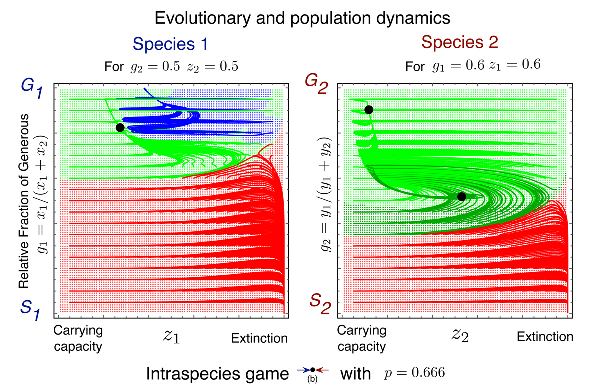
\includegraphics[width=\columnwidth]{Figures/mainexamplepopdyn2.pdf}
\caption{\small{
\textbf{Dynamics of evolutionary strategies and population density for an intraspecies coexistence game with interspecies mutualism.}
With exactly the same parameters as that of Figure \ref{fig:mainexampleone} with  symmetric death rates $e_1 = e_2 = 0.05$ we show two different numerically evaluated examples.
Left Panel: shows the outcomes in species $1$ when starting from $0.5$ fraction of ``Generous" individuals in species $2$ at half carrying capacity $z_2 = 0.5$.
While most of the initial conditions lead to an extinction of species $1$ (red), there exists a fixed point which can be reached when most of species $1$ is ``Generous" and close to carrying capacity (green). For the same or higher fraction of $G_1$ but lower population density, species $1$ can end up being completely ``Generous" (blue).
Right Panel: shows the outcomes in species $2$ when starting from $0.6$ fraction of ``Generous" individuals in species $1$ with empty spaces proportion of $z_1 = 0.6$.
When species $2$ is mostly made up of ``Selfish" types then it leads to species extinction (red), For intermediate levels of ``Generous"individuals there exists an internal equilibrium (dark green). However another stable equilibrium exists as well as even higher densities of ``Generous" types closer to full carrying capacity (green).
Equilibrium selection is thus possible for species $2$ in this case where it is preferable to have an intermediate number of ``Selfish" types.
\label{fig:popdyn}
}
}
\end{center}
\end{figure}



\section{Discussion}

Mutualistic interactions have been implicated as one possible mechanism facilitating the success of invasive species \citep{richardson:BR:2000}.
However mutualism based invasions also have the possibility to change the composition of the supporting local species.
About 150 ant species have been found invading new habitats mostly by forming mutualistic associations with honeydew producers \citep{mcglynn:JB:1999}.

Usually when interspecies relationships such as mutualism (or antagonist relationships as in predator-prey) are considered, the within species interactions are ignored for the sake of convenience.
The converse is the case when the intraspecies interactions are of interest.
The major body of work focusing on within population social dilemmas between Cooperators" and Defectors" is an example of the same.
Obviously, this is an assumption which is very useful when distilling the interactions at different community scales.
However when the inter and intraspecies interactions are interdependent then the feedbacks between the two levels cannot be ignored \citep{schluter:PlosB:2012}.

In principle the framework developed herein is capable of handling a diverse array of inter and intraspecific interactions.
For interspecific interactions our focus is on mutualism.
Mutualistic interactions between two species can be represented by a bimatrix game.
The components of each of the two game matrices need not be correlated as long as they independently satisfy the inequalities leading to a Snowdrift games. 
Including realistic phenomena such as intraspecies interactions, population dynamics and seasonality we show that maintenance of mutualism is possible.
A fragile balance of parameters maintains mutualism. 
If within each species the ``Generous" and ``Selfish" interactions result in coexistence then it can outweigh the competition which they experience at the interspecies level.
Note however that at the interspecies level the competition of a ``Generous" individuals is with the ``Selfish" individuals from the other species. 
While the ``Selfish" individuals from the other species can drive ``Generous" individuals within a species extinct, co-existence between ``Generous" and ``Selfish" within the same species can overcome the pressure for extinction. 
In this way, mutualism can be maintained but it comes at a cost of also maintaining a significant level of exploiters. 
In fact the coevolutionary dynamics between the two species is determined together by the inter as well as the intraspecific interactions.

While the simple case makes predictions possible, including seasonality inserts a time dependent factor which makes analytical reasoning difficult.
However given the patterns of episodic interactions and studies of mutualistic relationship obtained from field studies over the decades it might be possible to include the seasonal component in future analysis on realistic systems to see how the interactions are going to change under drastic climate change.
Including this feature informs us of the dependence of the mutualism on environmental factors.
This is particularly important as species specific mutualisms are at a high risk of being destabilised.
For example bird pollinators of numerous plants are sensitive to the environmental and ecological changes which can occur naturally or catalysed by anthropogenic activity.
The difference in the timescales of the evolutionary process and environmental fluctuations highlights the fact that averaging out the environmental effects might not always be possible.
The system can show qualitatively different behaviour from the average dynamics depending on the kind of interactions initially involved within and between species.

An ecologically important example of species specific mutualism is that of sunbirds, particularly the Malachite Sunbird (\textit{Nectarine famosa}) and the geophyte \textit{Brunsvigia littoralis}.
Besides being sensitive to the environmental variation, \textit{B. littoralis} it furthermore suffers from low population densities \citep{geerts:SAJB:2012} and threatened by rapid urbanisation.
An example more economically connected to humans comes from the honeybee, \textit{Apis mellifera}.
A species of immense capital importance, the colony collapse of this pollinator has been attributed to numerous causes ranging from the pesticides to biological interference from parasites and pathogens as well as a change in the environment \citep{nazzi:PLosPath:2012}.

Our framework incorporates exactly these essential elements of interspecies interactions and changing environments, predicting a deep impact on population dynamics of the interactors.
While our focus is currently on mutualism, it is easy to change the interactions by changing/modifying the game defining the interspecies interactions.
Including population dynamics and the real threat of extinction needs to be acknowledged when modelling such scenarios.
Only then can better conservation tactics be formulated which are not solely based on evolutionary predictions but eco-evolutionary dynamics.

Going back to one of the most well studied examples of mutualism, the squid-vibrio symbiosis, it is hard to exclude population dynamics at least from one of the interacting species \citep{nyholm:NRM:2004}.
The diel pattern of the host squid is associated with oscillations in the population density of the symbiont \textit{Vibrio fiscerei}.
Since the growth rates of the two species differ vastly, the population size turnover inside the squid needs to be managed.
While the squid makes use of the full light organ at night camouflaging itself from predators, at dawn it expels almost $95\%$ of the bacteria.
The squid lies buried underground during the day and the remaining $5\%$ of the bacteria repopulate the light organ again reaching saturation by mid-afternoon.
While in our model the population dynamics of the mutualists are driven by the empty spaces in their own niches, this particular example beckons a specific modeling approach where the host itself acts as the niche environment of the symbiont and controls the population density too.
Since this determines the viability or extinction of a species, it is not a trivial feature which can be excluded when understanding mutualism.
Our framework comes with the capability of including such specific examples and can be modified to suit particular examples.
It thus helps in not only elucidating the interactions which might be involved in generating the dynamics which we observe in nature but rather provide the criteria under which the observed dynamics are being maintained and ways to explore their stability under varying crucial parameters. 

Our study shows the critical nature of mutualism and the sliver of parameter space where they are maintained. 
A slight change in the values can either end up in a system where one of the mutualist is completely exploited by the other species or even leads to extinction of both types in case of obligate mutualisms.
Going back to \cite{janzen:bookchapter:1985} an appropriately succinct summary would be,
`A mutualist today may be a parasite of the mutualism tomorrow'.

\textbf{Acknowledgements}. \cha{CSG acknowledges funding from the New Zealand Institute for Advanced Study and time spent at Victoria University of Wellington. \ldots }


\bibliographystyle{plainnat}
%\bibliographystyle{mdpi}

\bibliography{\string~/Bibtex/et.bib}




\renewcommand{\theequation}{A.\arabic{equation}}
\setcounter{equation}{0}

\renewcommand{\thefigure}{A.\arabic{figure}}
\setcounter{figure}{0}

\begin{appendices}

\section{Interspecies Evolutionary Dynamics}

Traditional coevolutionary models consider interspecific dependence only \citep{roughgarden:TPB:1976,roughgarden:book:1983}.
Since in our case each the interactions between the species are mutualistic and each species consists of two types of individuals ``Generous" and ``Selfish", the following Snowdrift game is an appropriate representation of the interactions.
%This is because we have neglected intraspecific interactions as mentioned earlier.

%For different types of interactions between species different models need to be defined \citep{poulin:JTB:1995,doebeli:PNAS:1998,noe:book:2001,johnstone:ECL:2002,bergstrom:PNAS:2003,hoeksema:AmNat:2003,akcay:PRSB:2007,bshary:Nature:2008}.




\subsection*{The snowdrift game}
\label{appA}
\subsubsection*{Two player setting}
%So far, we have described general games within and between species, now we turn to a particular game which of interest to us when considering mutualism.
Two drivers are stuck in a snowdrift.
They must shovel away the snow (paying the cost $c$) to reach home (benefit $b$) but there are three possible outcomes to this scenario.
One of the driver shovels while the other stays warm in the care ($b-c$ and $b$), both the drivers share the workload and shovel away the snow ($b-c/2$ and $b-c/2$) or none of them gets out of the care and they both remain stuck ($0$ and $0$).

Putting this game in perspective of the two species (i.e. the two drivers represent the two different species) we get the matrix,\\
%
\begin{equation}\label{}
\begin{array}{cc|cc}
\multicolumn{4}{l}{\textit{Species 1 payoff:}} \\
\hline\hline
& & \multicolumn{2}{c}{\text{Species 2}}\\
&	&	G_2		&	S_2	\\
\hline
 \multirow{2}{*}{Species 1} & G_1 	& b-c/2 &	b-c \\
&	S_1	&  b & 0 \\
 \hline\hline
\end{array}
\hspace{1cm}
\begin{array}{cc|cc}
\multicolumn{4}{l}{\textit{Species 2 payoff:}} \\
\hline\hline
& & \multicolumn{2}{c}{\text{Species 1}}\\
&	&	G_1		&	S_1	\\
\hline
 \multirow{2}{*}{Species 2} & G_2 	& b-c/2 &	b-c \\
&	S_2	& b & 0  \\
 \hline\hline
\end{array}
\end{equation}
%
where strategy $G$ stands for being \textit{``Generous"} and shoveling the snow while $S$ stands for being \textit{``Selfish"} and just sitting in the car.
For $b=2$ and $c=1$ we recover the matrix used in \citep{bergstrom:PNAS:2003}.

For the snowdrift game in a single population for which the pairings are formed at random, there exists a single, stable internal equilibrium.
Hence the population will evolve to a polymorphism which is a combination of \textit{``Generous"} and \textit{``Selfish"} individuals.
But in a two species system (pairs still random, but one from each species), this stable equilibrium turns into a saddle point: a small deviation from this fixed point leads the system to one of the stable fixed point where one of the species is completely \textit{``Generous"} and the other one is completely \textit{``Selfish"}.

\subsection*{Multiplayer setting}


Following Souza et al. \citep{souza:JTB:2009},  
a multiplayer snowdrift game can be described by the payoff entries
\begin{eqnarray}
\Pi_{G_1} (k)  &=& \begin{cases} b-\frac{c}{k} & \textrm{if } k \geq M \\  -\frac{c}{M} & \textrm{if } k < M \end{cases} 
\\
\Pi_{S_1} (k)  &=& \begin{cases} b & \textrm{if } k \geq M \\ 0 & \textrm{if } k < M. \end{cases}
\label{eqintergamepayoffs}
\end{eqnarray}
%
All players get the benefit $b$ if the number of generous individuals in both species combined, $k$, is greater than or equal to the threshold $M$.
For the generous individuals, their effort is subtracted from the payoffs.
The effort is shared if the quorum size is met ($\frac{c}{M}$), but is in vain for $k<M$. 
For two player games we had $k=1$ but multiplayer games provide the possibility of exploring this threshold aspect of collective action games.
From these payoff entries we need to calculate the average fitnesses.
For simplicity we just illustrate the fitnesses of the strategies in species $1$.
For a $d_1^{inter}$ player game for species $1$ we need to pick $d_1^{inter}-1$ other individuals from species $2$.
Assuming random sampling the composition of the formed groups is given by a binomial distribution.
Summing over all possible compositions of groups we arrive at  the average fitnesses of the two strategies in species $1$,
%
\begin{align}
f^{inter}_{G_1} (y) &= \sum_{k=0}^{d_1^{inter} -1} \binom{d_1^{inter} -1}{k}y^k (1-y)^{d_1^{inter} -1-k} \Pi_{G_1}(k+1)  \\
f^{inter}_{S_1} (y) &= \sum_{k=0}^{d_1^{inter} -1} \binom{d_1^{inter} -1}{k}y^k (1-y)^{d_1^{inter} -1-k} \Pi_{S_1}(k),
\label{interfiteqs}
\end{align}
%
and similarly $f_{G_2}^inter$ and $f_{S_2}^inter$ for species $2$.

Note that here for the sake of notation we have assumed the same values of benefits and costs, thresholds for the two species. However along with the number of player $d_1^{inter}$ and $d_2^{inter}$, these parameters could be very well different for the two species.
For asymmetric bi-matrix games there is a difference in the dynamics between the standard replicator dynamics and the alternative dynamics put forward by Maynard-Smith \citep{maynard-smith:book:1982}.
In this case the replicator equations cannot be simplified by removing the average fitness from the denominator and can give rise to qualitatively different dynamics. 
Then one has to resort to difference rather than differential equations.

\section{Intraspecies Evolutionary Dynamics}
\label{appB}

For elucidating the intraspecies dynamics we will focus on species $1$ as the analysis is analogous for species $2$.
Within species dynamics can in principle be completely different from the between species interactions. 
We can have a multistrategy multiplayer game within a species but to keep things simple we assume a two strategy multiplayer game.
The partitioning of the individuals into two strategies follows the same partitioning as in the inter species interactions as of ``Generous" and ``Selfish". 
In principle we could have two different labels for the strategies in the intraspecies interactions and the ``Generous" and ``Selfish" categories could be split into them.
However for the sake of simplicity we assume the same categorisation as at the inter species level.

\subsection*{Synergy/Discounting Framework}
We model the within species interactions by making use of a general framework of costs and non-linear benefits \citep{eshel:AmNat:1988,hauert:JTB:2006a} which can potentially encompass all different types of (traditionally studied) social interaction structures qualitatively \citep{nowak:book:2006}, i.e., dominance of either type, coexistence and bistability.
Since the categorisation of the strategies at the intraspecies level is the same as that of the inter species level, for species $1$, $x$ and $1-x$, are the frequencies of ``Generous" and ``Selfish" type. 
The ``Generous" and ``Selfish" in species $1$ play a $d_1^{intra}$ player game.
Thus the fitnesses of of the two types are defined as \citep{hauert:JTB:2006a},
%
\begin{align}
	f^{intra}_{G_1} (x) &= \sum_{k=0}^{d_1^{intra} -1} \binom{d_1^{intra} -1}{k}x^k (1-x)^{d_1^{intra} -1-k} \Gamma_{G_1}(k+1)  \\
	f^{intra}_{S_1} (x) &= \sum_{k=0}^{d_1^{intra} -1} \binom{d_1^{intra} -1}{k}x^k (1-x)^{d_1^{intra} -1-k} \Gamma_{S_1}(k).
\label{intrafiteqs}
\end{align}
%
where the payoffs are given by,
\begin{align}
	\Gamma_{S_1} (k) = \frac{\tilde{b}}{d_1^{intra}} \sum_{i=0}^{k-1} \omega^i  \\
	\Gamma_{G_1} (k) = \Gamma_{S_1} (k) - \tilde{c}.
\label{eqintragamepayoffs}
\end{align}
%
Thus the ``Selfish" get a fraction of the benefit which is scaled by the factor $\omega$, which determines whether the benefits are linearly accumulating ($\omega=1$) for increasing number of ``Generous" individuals, synergistically enhanced ($\omega>1$) or saturating ($\omega<1$).
Note that the costs and benefits in the within species game need not be the same as in between species ($b\neq \tilde{b}$ and $c \neq \tilde{c}$).


\section{Combined Evolutionary Dynamics}
\label{app:combineddyn}

The average payoffs are then assumed to be a linear combination of the interspecies and intraspecies interactions where the parameter $p$ determines the strength of each of the interactions such that,
%
\begin{align}
	f_{G_1} (x,y) &= p f^{inter}_{G_1} (y) + (1-p) f^{intra}_{G_1} (x)  \\
	f_{S_1} (x,y) &= p f^{inter}_{S_1} (y) + (1-p) f^{intra}_{S_1} (x).
\label{fiteqs}
\end{align}
%
Following the same procedure for the two strategies in species $2$ leads to the average fitness
%
\begin{align}
\bar{f}_1 (x,y) &= x f_{G_1} (x,y)+(1-x) f_ {S_1}(x,y)  \\
\bar{f}_2 (x,y) &= y f_{G_2} (x,y)+(1-y) f_{S_2}(x,y).
\label{avgfiteqs}
\end{align}
%
The time evolution of the ``Generous" types in both the species will give us the complete dynamics of the system.
However since the two interaction species are by definition different organisms, they can have different rates of evolution.
Thus if species 1 evolves at the rate $r_x$ while species 2 at rate $r_y$ then we have,
\begin{align}
\dot{x} &= r_x x \left(f_{G_1}(x,y) -  \bar{f}_1(x,y) \right)  \\
\dot{y} &= r_y y \left(f_{G_2}(x,y) -  \bar{f}_2(x,y) \right).
\label{eq:repeqapp}
\end{align}


\begin{sidewaysfigure}[ht]
    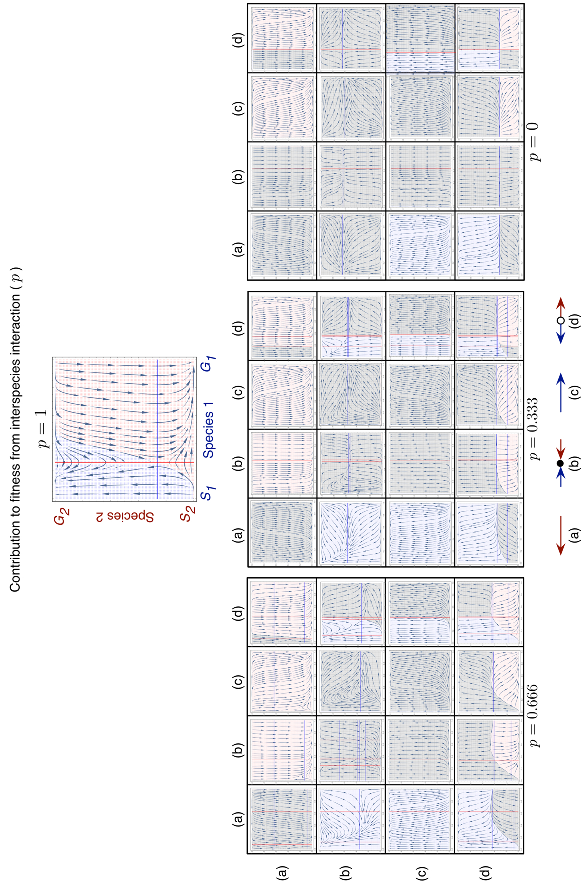
\includegraphics[width=\columnwidth]{../Figures/Dynamicsacrossp_reduced.pdf}
    \caption{
$d_1^{inter} = d_2^{inter} = 5$, $b = 2$, $r_x = r_y/8$, $M_1 = M_2 = 1$ and $c=1$ for the interspecies game. As for the intraspecies games we have $d_1^{intra} = d_2^{intra} = 5$ and $\tilde{b} = 10 $ with 
(a) $\tilde{c} = 3$, $\omega = 3/4$, 
(b) $\tilde{c} = 1$, $\omega = 3/4$, 
(c) $\tilde{c} = 1$, $\omega = 4/3$ and 
(d) $\tilde{c} = 3$, $\omega = 4/3$, the exact same parameter values as in \citep{hauert:JTB:2006a}.
\label{fig:appendix}
}
\end{sidewaysfigure}


%\begin{figure}[h]
%\begin{center}
%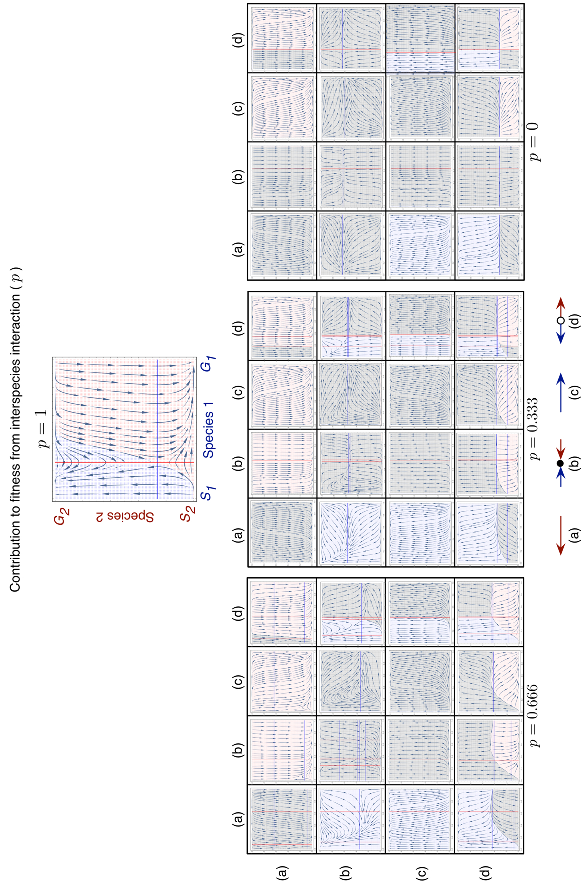
\includegraphics[width=\columnwidth]{../Figures/Dynamicsacrossp_reduced.pdf}
%\caption{
%$d_1^{inter} = d_2^{inter} = 5$, $b = 2$, $r_x = r_y/8$, $M_1 = M_2 = 1$ and $c=1$ for the interspecies game. As for the intraspecies games we have $d_1^{intra} = d_2^{intra} = 5$ and $\tilde{b} = 10 $ with 
%(a) $\tilde{c} = 3$, $\omega = 3/4$, 
%(b) $\tilde{c} = 1$, $\omega = 3/4$, 
%(c) $\tilde{c} = 1$, $\omega = 4/3$ and 
%(d) $\tilde{c} = 3$, $\omega = 4/3$, the exact same parameter values as in \citep{hauert:JTB:2006a}.
%\label{fig:appendix}
%}
%\end{center}
%\end{figure}


%\cha{\section*{Asymmetries}}
%
%\cha{This between and within species model is a powerful way of introducing a lot of variability into the dynamics,
%\begin{align}
%	d_1 &\neq d_2 \\
%	d^{inter} &\neq d^{intra} \\
%	M_1 &\neq M_2 \\
%	b &\neq \tilde{b} \\
%	c &\neq \tilde{c} \\
%	r_x &\neq r_y \\
%	&\vdots
%\end{align}
%and various combinations of these. We should justify why we don't do this here and why we do vary the ones that we do.}


%\subsection{Dynamics in asymmetric conditions}
%
%%We have addressed two kinds of asymmetries in the game, the number of player and the thresholds in the two species.
%%We denote the number of players for species $1$ and species $2$ as $d_1$ and $d_2$, respectively, as in Fig.\ \ref{fig:counter}.
%%That is if species $2$ is playing a $d_2$ player game it means that one player from species $2$ interacts with $d_2-1$ players of species $1$.
%%For an asymmetry in the thresholds we use the two parameters $M_1\geq1$ and $M_2\geq1$ for the two species, respectively.
%
%For asymmetric bimatrix games, there is a difference in the dynamics between the standard replicator dynamics and the 
%alternative dynamics put forward by Maynard-Smith \citep{maynard-smith:1982to}.
%For this dynamics, the average fitness of each species appears as a denominator,
%\begin{align}
%\dot{x} &= r_x x \left(f_{G_1}(y) -  \bar{f}_1(x,y) \right)/\bar{f}_1(x,y)  \\
%\dot{y} &= r_y y \left(f_{G_2}(x) -  \bar{f}_2(x,y) \right)/\bar{f}_2(x,y).
%\label{eq:repeqs}
%\end{align}
%In our asymmetric bimatrix game, the fixed point stability is affected by the choice of the dynamics, in contrast to the case of symmetric games. 
%%In Fig.\ \ref{fig:thresholdsmodrep}, we illustrate that the dynamics is different between the usual replicator dynamics and Eqs. \ref{eq:repeqs}
%
%For $d_1=d_2 \geq 5$, the exact coordinates of the fixed point must be computed numerically \citep{abel:AO:1824,stewart:book:2004}.


\section{Population dynamics}

For brevity we begin with the description of population dynamics in species 1.
The two types in species 1, ``Generous" and ``Selfish" need not sum up to $1$ i.e. the population may not always be at its carrying capacity.
Hence if the empty space in the niche occupied by species $1$ is $z_1$, then we have $x_1 + x_2 + z_1 = $ where $x_1$ and $x_2$ are the densities of ``Generous" and ``Selfish" types.
The population dynamics then is dictated by,
%
\begin{align}
	\dot{x_1} &= r_x x_1 (z_1 f_{G_1} - e_1)  \\
	\dot{x_2} &= r_x x_2 (z_1 f_{S_1} - e_1) \\
	\dot{z_1} &= - \dot{x_1} - \dot{x_2} 
\end{align}
%
and for species 2
\begin{align}
	\dot{y_1} &= r_y y_1 (z_2 f_{G_2} - e_2)  \\
	\dot{y_2} &= r_y y_2 (z_2 f_{S_2} - e_2) \\
	\dot{z_2} &= - \dot{y_1} - \dot{y_2} 
\end{align}
%
We have $e_1$ and $e_2$ as the death rates for the two species. 
For the special case of  $e_1 = \frac{z_1 (x_1 f_{x_1} + x_2 f_{x_2}) }{x_1 + x_2}$ and $e_2 = \frac{z_2 (y_1 f_{G_2} + y_2 f_{S_2}) }{y_1 + y_2}$ we recover the two species replicator dynamics as in Eqs.~\ref{eq:repeqapp}. 
The fitnesses however need to be reevaluated in this setup.
For example in species 1 the fitness for type $G_1$ is,
%
\begin{align}
	f_{G_1}^{inter} &= \sum_{S=2}^{d_1} \binom{d_1 -1}{S-1} z_2 ^{d_1 -S} (1-z_2)^{S-1} P_G^{inter}(S,y_1,y_2,z_2) \\
	f_{G_1}^{intra} &= \sum_{S=2}^{d_1} \binom{d_1 -1}{S-1} z_1 ^{d_1 -S} (1-z_1)^{S-1} P_G^{intra}(S,x_1,x_2,z_1) \\
	f_{G_1} &= f_{G_1}^{inter} + f_{G_1}^{intra}
\end{align}
%
and similarly for type $S_1$ where the payoff functions are defined as,
%
\begin{align}
	P_G^{inter}(S,p,q,r) &= \sum_{k=0}^{S-1} V(S,p,q,r) \Pi_{G_1}(k+1) \\
	P_G^{intra}(S,p,q,r) &= \sum_{k=0}^{S-1} V(S,p,q,r) \Gamma_{G_1}(k+1) \\
	P_S^{inter}(S,p,q,r) &= \sum_{k=0}^{S-1} V(S,p,q,r) \Pi_{S_1}(k) \\
	P_S^{intra}(S,p,q,r) &= \sum_{k=0}^{S-1} V(S,p,q,r) \Gamma_{S_1}(k)
\end{align}
%
where $V(S,p,q,r) = \binom{S-1}{k} \left( \frac{p}{1-r}\right)^k  \left(\frac{q}{1-r}\right)^{S-1-k}$ is the probability of having a $k$ ``Generous"(Cooperator) individuals and $S-1-k$ ``Selfish"(Defector) individuals in the inter(intra) species game.
and the actual payoffs are calculated as per Eqs.~\ref{eqintergamepayoffs} and \ref{eqintragamepayoffs}.

\end{appendices}

\end{document}